\section{Discussion}

\paragraph{Choosing a width.}
For Gemma 3 sizes 4B and larger, choose widths 1/32 to 1/128, since they beat 1/4 in excess agreement at both 2,000 and 4,000 epochs, even when using live-only excess agreement (Section~4.2).
Held-out fit (explained variance on test rows) at these sizes varies by at most 0.011 across the six main widths, and at 2,000 epochs, training-row fit falls by 0.285 to 0.329 from 1/4 to 1/128 (Appendix~D).
For 270M and 1B, no main width has more than 2.6\% and 7.7\% of meta-latents recurring, respectively.

\begin{figure}[t]
  \centering
  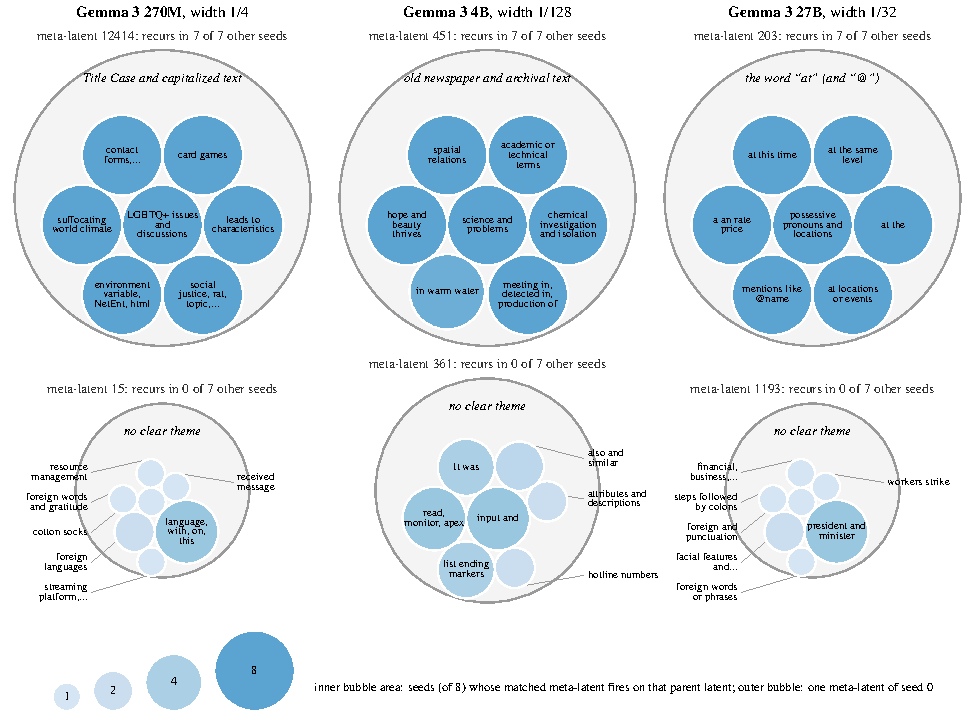
\includegraphics[width=\linewidth]{figures/examples.pdf}
  \caption{Example seed-0 meta-latents that recur in all seven other seeds (top) or in none (bottom), with their seven most strongly activating parent latents and Neuronpedia's automatic labels \citep{lin2023neuronpedia}. Italic descriptions come from three blinded AI readers.}
  \label{fig:examples}
\end{figure}

\paragraph{What the uses rely on.}
Interpretability practitioners commonly analyze individual meta-latents \citep{bussmann2024metasae,leask2025canonical,zhao2026saepp}, and such analyses rely on those meta-latents recurring.
At the main near-best widths for our setups of sizes 4B and larger at 2k epochs, 18.3\% to 27.4\% (19.2\% to 29.9\% at 4k epochs) of meta-latents recur.
At the top main widths for 270M, 4B, and 27B, Figure~\ref{fig:examples} shows the seed-0 meta-latent that recurs in the seven other seeds and also the meta-latent that recurs in none---each chosen as the middle of its group by number of parent latents activated on.
The top parent latents of the recurring meta-latents are activated on in seven to eight of the eight seeds while those for the nonrecurring meta-latents are activated on in at most five, meaning analyses of the nonrecurring meta-latents may not carry over to another seed.
\citet{korznikov2025ortsae} also analyze explained variance of the parent decoder weights, but describe no held-out split.
We found that at \citeauthor{korznikov2025ortsae}'s \citeyearpar{korznikov2025ortsae} width (1/4), our real meta-SAEs explain 4.1 to 5.9 times as much variance on training rows as on test rows (Appendix~D).
We also argue others should prefer excess agreement over raw agreement.

\paragraph{Why.}
Across the five main sweep parents, fewer parent latents per hidden dimension seems to correlate with higher excess agreement, and the 4B 16k parent scores above the 4B 65k parent as this would predict, but the 270M 16k and GPT-2 parents do not fit this trend.
We do not claim to know why the real meta-SAEs agree less than their noise twins at narrow widths for 270M and 1B (Section~4.1) and for the 270M 16k control (Section~4.3), but one hypothesis we offer---with the exception of the GPT-2 parent-based setup---is that the two smallest Gemma 3 models, with their text-only input and small hidden sizes, cannot represent enough broad concepts for a narrow meta-SAE to group the parent's latents as consistently across seeds as a noise twin does by settling along its covariance.
In every main setup, real meta-SAEs fit the test rows better than their noise twins do, but we did not measure how much of that gap comes from the shift in the twins' statistics (Section~3).

\paragraph{Prior findings.}
Our findings of narrower widths of meta-SAEs winning for Gemma 3 4B and larger are similar to how \citet{paulo2025sae} observed SAEs with fewer latents having more seed-to-seed agreement.
Note that their 30\% counts a latent only when both its encoder and decoder match at cosine 0.7, whereas our 29.9\% only counts decoder matches on meta-SAEs.
Also, unlike \citeauthor{liu2026timescale}'s \citeyearpar{liu2026timescale} finding that longer training makes SAE widths more alike in mean max cosine similarity (MMCS, relative to an analytic random-dictionary reference), the top meta-SAE width's lead over 1/4 in excess agreement grows at 12B and 27B from 500 to 4k epochs, shrinking only at 4B (Figure~\ref{fig:length}).
